% !TEX root = ../main.tex

\section{Introduction} \label{sec:intro}

Blockchain technology enables smart contracts or decentralized applications (DApps). Function calls (or transactions) to the DApp are processed by a decentralized network. Transactions are finalized in stages: they (generally) first relay around the network, then are selected by a miner and put into a valid block, and finally the block is well-enough incorporated that is unlikely to be reorganized. Front-running is an attack where a malicious node observes a transaction after it is broadcast but before it is finalized, and attempts to have its own transaction confirmed before or instead of the observed transaction. 

The mechanics of frontrunning works on all DApps but front-running is not necessarily beneficial, depending on the DApp's internal logic and/or  as any mitigations it might implement. Therefore DApps need to be studied individually or in categories. This paper is a series of case studies of DApps deployed on Ethereum (a popular blockchain supporting DApps) from each category of the top 25 most active.\footnote{List of decentralized applications \url{https://DAppradar.com/DApps}} We do case studies on decentralized exchanges (\eg Bancor), crypto-collectables (\eg CryptoKitties), gambling services (\eg Fomo3D), and decentralized name services (\eg Ethereum Name Service). We also study initial coin offerings (ICOs), which by happenstance, did not appear in the top 25 on our sample day. After a few hacking incidents of high valued smart contracts~\cite{siegel2016daohack}, ICOs started to implement restrictions and capped how much funds can be gathered. This scarcity of the initial coins made for a competition to incentivize big investors to get in and buy the tokens at a discounted price and sell them to latecomers on the open markets~\cite{zetzsche2018ico, li2018initial}. ICOs started to experiment with different fair capping methods, such as reverse dutch auction and dynamic ceilings~\cite{kaal2017initial}. We show empirical evidence of a miner purchasing tokens ahead of other users in Status.im. Finally, proposals to eliminate or mitigate frontrunning from DApps are scattered across forums, proposed standards (called EIPs in Ethereum) and academic papers; we systemize them the last section. 

% = = = = = = = = = = = = = = = = = = = = = = = = = = %
% = = = Preliminaries
% = = = = = = = = = = = = = = = = = = = = = = = = = = %

\section{Preliminaries \& Related Work}

\subsection{Traditional Front-running} 
\label{sec:What is front-running?}

\emph{Front-running} is a course of action where someone benefits from early access to market information about upcoming transactions and trades, typically because of a privileged position along the transmission of this information. The problem can occur in both financial and non-financial systems. In traditional stock exchanges, floor traders might overhear a broker's negotiation with her client over a large purchase, and literally race the broker to buy first, potentially profiting when the large sale temporarily reduces supply of the stock. A malicious broker might also front-run their own client's orders by purchasing stock for themselves between receiving the instruction to purchase from the client and actually executing the purchase (similar techniques can be used for large sell orders). Front-running is unethical and illegal in jurisdictions with mature securities regulation. 

Cases of front-running are sometimes difficult to distinguish from related concepts like insider trading and arbitrage. In front-running, a person sees a concrete transaction that is set to execute and reacts to it before it actually executes. If the person instead has access to more general privileged information that might predict future transactions, but is not reacting at the actual pending trades, we would classify this activity as insider trading. If the person reacts after the trade is executed, or information is made public, and profits from being the fastest to react, this is considered arbitrage and is both legal and encouraged because it helps markets integrate new information into prices quickly.

\subsection{Literature on Traditional Front-running}\label{traditionalFrontrunning}
Front-running was first observed on the Chicago Board Options Exchange (\textit{CBoE})~\cite{markham1988front}, and was defined by Securities Exchange Commission \textit{(SEC)} in 1977 as: ``The practice of effecting an options transaction based upon non-public information regarding an impending block transaction\footnote{Block in the stock market is a large number of shares, 10\,000 or more, to sell which will heavily changes the price} in the underlying stock, in order to obtain a profit when the options market adjusts to the price at which the block trades.~\cite{sec1978optionsmarket}''

Self-regulating exchanges (\eg \textit{CBoE}) and the \textit{SEC} spent the ensuing years planning how to detect and outlaw front-running practices~\cite{markham1988front}. The \textit{SEC} stated: ``It seems evident that such behaviour on the part of persons with knowledge of imminent transactions which will likely affect the price of the derivative security constitutes an unfair use of such knowledge.\footnote{Securities Exchange Act Release No. 14156, November 19, 1977, (Letter from George A. Fitzsimmons, Secretary, Securities, and Exchange Commission to Joseph W. Sullivan, President  CBoE).}'' The \textit{CBoE} tried to educate their members on existing rules, however differences in opinion regarding the unfairness of front-running activities, insufficient exchange rules and lack of a precise definition in this area resulted in no action by self-regulator organizations~\cite{sec1978optionsmarket}. 

We refer the reader interested in further details on the early regulatory history of front-running to Markham~\cite{markham1988front}. Initially front-running policies applied only to certain option markets. In 2002, the rule was expanded to cover all security futures~\cite{finra_2002}. In 2012, it was expanded further with the new amendment, FINRA Rule 5270, to cover trading in options, derivatives, or other financial instruments overlying a security with only a few exceptions~\cite{sec2012frontrunning, finra_2012}.

\subsection{Background on Blockchain Front-running} \label{sec:Front Running on the Blockchains}

In one sense, blockchain technology (which was introduced via Bitcoin in 2008~\cite{nakamoto2008bitcoin}) strives to disintermediate certain central parties that would participate in a transaction. However, blockchains also introduce new participants in the relaying and finalization (\ie mining) of transactions that can act as front-runners. Any user monitoring blockchain network transactions (\eg running a full node) can see a unconfirmed transactions and broadcast a reactionary transaction that might be confirmed ahead of the original transaction ... 

 that is well-connected front-run other transactions in the network. For regular users to front-run others on the blockchain, they need to be well connected to other nodes on the network. Doing so, they are able to listen to the network and monitor all transactions that are broadcast. On the Ethereum blockchain, users have to pay for the computations in a small amount of Ether called \textit{gas}~\cite{AccountT67:online}. The price that users pay for transactions, \textit{gasPrice}, can increase or decrease how quickly miners will execute them and include them within the blocks they mine. Once seeing two identical transactions with different transaction fees, a rational miner will prioritize the transaction that pays a higher gas price per unit of gas, \textsf{gasPrice}, due to limited space in the blocks. Therefore, any regular users who run a full-node Ethereum client can front-run pending transactions by sending similar transaction with higher gas price. Blockchain miners are the only parties who can decide on the order of transactions within a block they mine, they can easily intercept and reorder the transactions in their blocks, this in case of malicious reordering is known as \textbf{transaction reordering} attack. 

\subsection{Literature on Blockchain Front-running}

Aune~\etal discuss how the lack of time priority between broadcasting a transaction and its validation by miners on a blockchain based system would lead to market information leakage~\cite{aune2017footprints}.They also propose a cryptographic approach, similar to commit and reveal (see Section~\ref{CommitmentScheme}) to prevent front-running. Malinova and Park discuss different design settings for financial markets and trading platforms on decentralized ledgers~\cite{malinova2017market}. They argue that blockchain brings new options of transparency which affects traders behaviour, especially in the presence of intermediary front-runners. They model indirect trading costs and use the economic literature on search and trading at decentralized exchanges in their design settings to make front-running costly and inefficient. Breidenbach~\etal~\cite{breidenbach2018enter} face the front-running issue in the context of automating bug bounties for smart contracts. Upon submitting the bug bounty to the Hydra smart contract, one can front-run the bug report and claim the bounty instead of the original reporter. In order to mitigate this issue they proposed \textit{Submarine Commitments} which extend commit and reveal; we discuss them further in Section~\ref{submarineCommits}.

Double-spending attacks in Bitcoin have been studied~\cite{bamert2013have, karame2012double} where a user broadcasts a transaction and is able to obtain some off-blockchain good or service before the transaction has actually been (fully) confirmed. The user can then broadcast a competing transaction that sends the same unspent coins to herself, perhaps using higher transaction fees, arrangements with miners, or artefacts of the network topology to have the second transaction confirmed instead of the first. We think of this as a type of front-running.

In the cryptographic literature, front-running attacks are modelled by allowing a `rushing' adversary to interact with the protocol. In particular, ideal functionalities of blockchains (such as those used in simulation-based proofs) need to capture this adversarial capability, assuming the real blockchain does not address front-running. Literature like the Bitcoin Backbone~\cite{} and Hawk~\cite{} capture this. 

% = = = = = = = = = = = = = = = = = = = = = = = = = = %
% = = = TOP 25
% = = = = = = = = = = = = = = = = = = = = = = = = = = %

\section{Cases of Front-running in DApps}  
% !TEX root = ../main.tex

% ------------------------------------------------------------------------------------------------------------------------------------------------%
% Top 25 Dapps Table:%

\begin{table}[t]
\centering
\scriptsize
\begin{tabular}{|c|l|}

\hline
\textbf{DApp Category}    										& \textbf{Names (Ranking)} \\  \hline
\multirow{6}{*}{Exchanges} 										& IDEX (1) \\ 
															& \textbf{ForkDelta, EtherDelta} (2) \\
															& \textbf{Bancor} (7) \\
															& The Token Store (13) \\
															& LocalEthereum (14) \\
															& Kyber (22) \\ 
															& \textbf{0x Protocol} (23) \\ \hline

\multirow{9}{*}{\shortstack{Crypto-Collectible \\ Games \\ (ERC 721)}}		& \textbf{CryptoKitties} (3) \\  
															& Ethermon (4)\\
															& Cryptogirl (9)\\
															& Gods Unchained TCG (12)\\
															& Blockchain Cuties (15)\\
															& ETH.TOWN! (16)\\
															& 0xUniverse (18)\\
															& MLBCrypto Baseball (19)\\
															& HyperDragons (25)\\ \hline

					
\multirow{8}{*}{Gambling}											& \textbf{Fomo3D} (5) \\  
															& DailyDivs (6) \\																								& PoWH 3D (8)	 \\ 
															& FomoWar (10) \\
															& FairDapp (11)\\
															& Zethr (17) \\
															& dice2.win (20) \\ 
															& Ether Shrimp Farm (21) \\  \hline	

							
\multirow{1}{*}{Name Services}									& \textbf{Ethereum Name Service} (24)  \\  \hline	


\end{tabular}
\caption{\footnotesize{Top 25 DApps based on recent user activity from \texttt{DAppRadar.com} on September 4th, 2018. We discuss the DApps that are in bold.}\label{tab:top25DApps}}
\end{table}

%TODO: mention the ones in italic are the ones we talk about
% ------------------------------------------------------------------------------------------------------------------------------------------------%

To find example DApps to study, we use the top 25 DApps based on recent user activity from \texttt{DAppradar.com} and sampled it in in the first week of September 2018.\footnote{List of decentralized applications \url{https://DAppradar.com/DApps}} User activity is admittedly an imperfect metric for finding the `most significant' DApps: significant DApps might be lower volume overall or for extended periods of time (\eg ICOs, which we remedy by studying independently in Section~\ref{sec:ICOsfrontrunning}). However user activity is arguably the best objective criteria for which data is readily available, the list captures our intuition about which DApps are significant, and it is at least better than an ad hoc approach. Using the dataset, we categorized the top 25 applications into 4 principal use cases. The details are given in Table~\ref{tab:top25DApps}.

% = = =  

\subsection{Markets and Exchanges} \label{sec:frontrunningExchanges}

% talk about velocity that seems to be not front-runnable but because of the liquidity pool limitation, there can be an order that consumes the last chunk of liquidity ``edge case'', to front run others and make their "option calls" fail

%Tragedy of the commons

% can we talk about Velocity here? ~\cite{eskandari2017feasibility} As the smart contract is the entity that acts as the market maker on regular cases with high liquidity front-running of the option calls do not result in any advantages, however, in the case of low balance of smart contracts pool of funds, the front-runner can front-run others to use up the remaining of the funds and make the rest of the option calls fail. 

\begin{figure}[h]
\centering
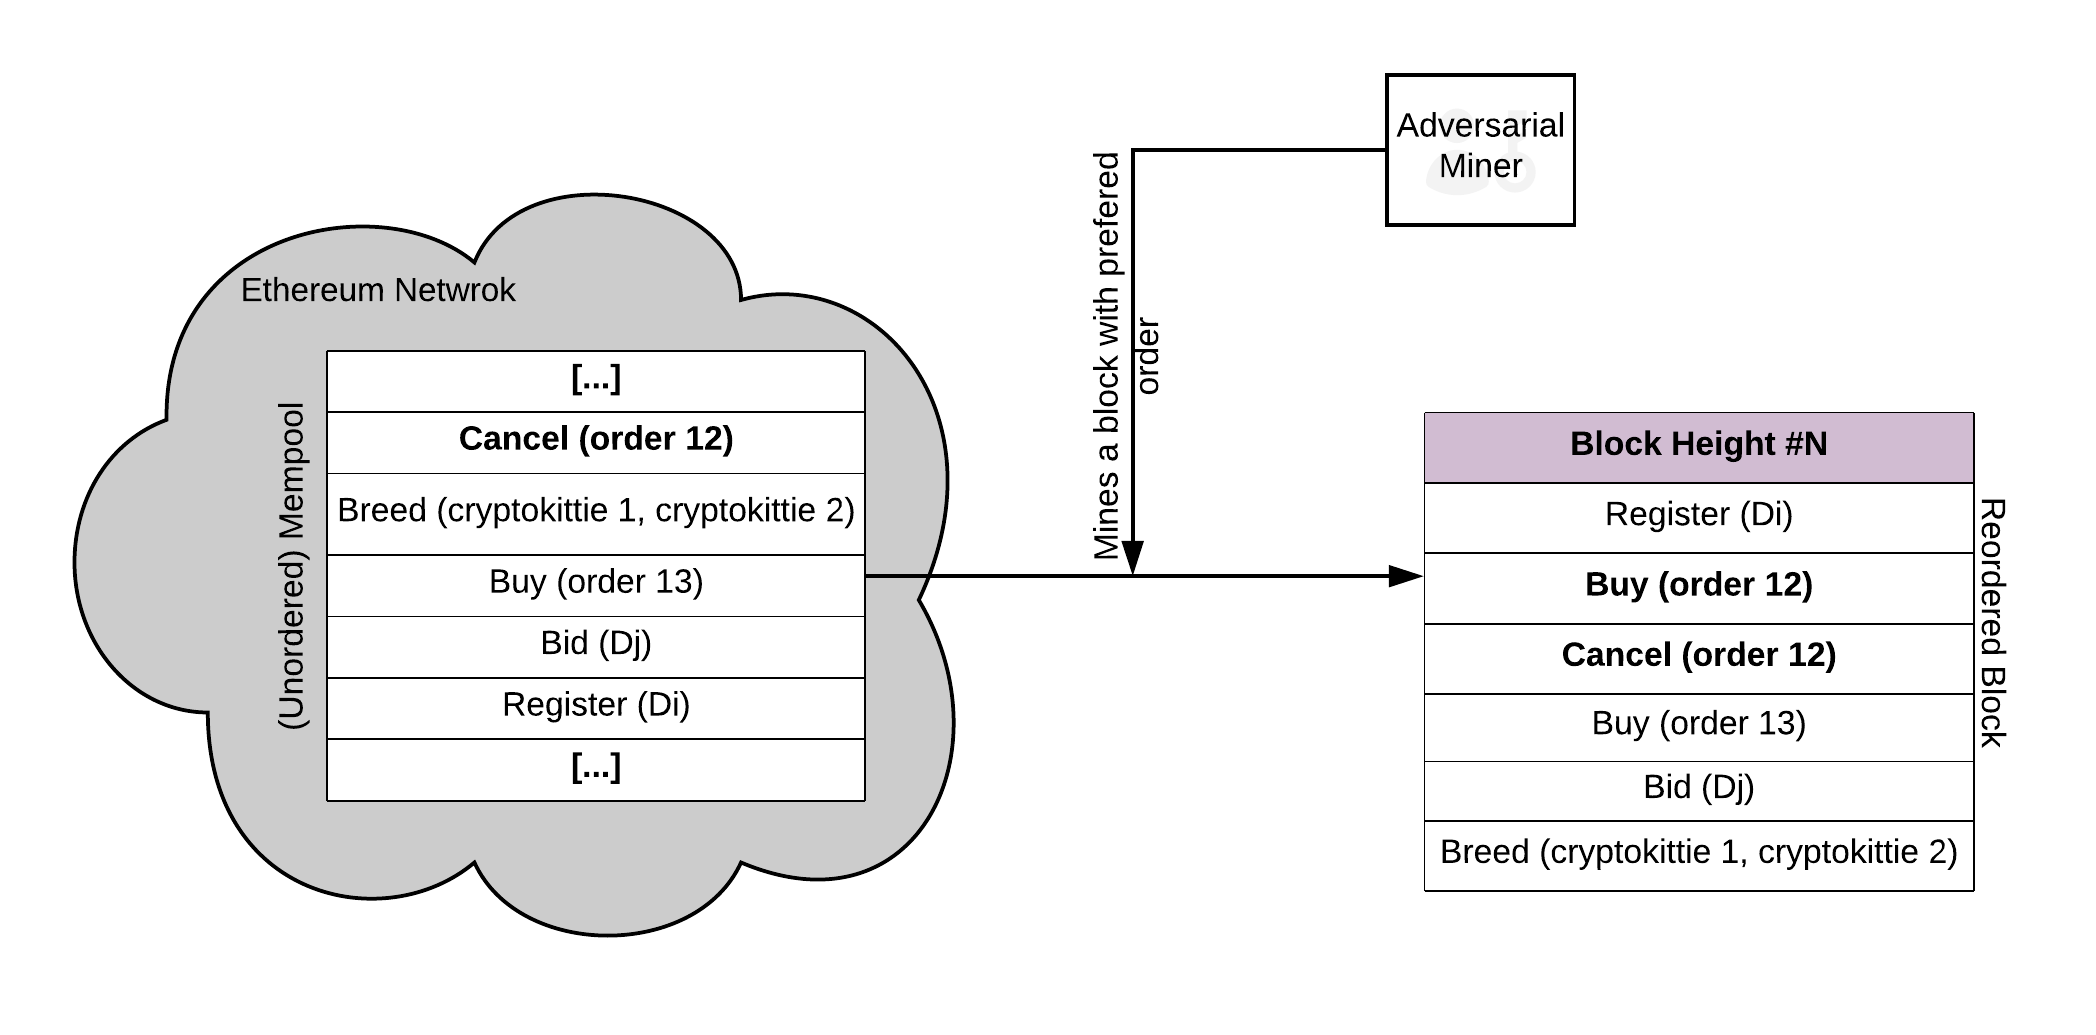
\includegraphics[width=0.7\linewidth]{figures/Miner_reorder_frontrun.png}
\caption{The adversarial miner can monitor the Ethereum mempool for decentralized exchange cancel orders and upon seeing the cancellation transaction, he puts his buy order prior to the cancel transaction. Doing so, the miner can profit from the underlying trade and also get the gas included in the cancel transaction. \label{fig:MinerFrontrunning}} 
\end{figure}
%https://www.lucidchart.com/invitations/accept/c8768786-4a3f-4c78-b3c8-aa04a6b81d06

The first category of DApp in Table~\ref{tab:top25DApps} is exchanges. Exchanges such as EtherDelta\footnote{also known as ForkDelta for the UI \url{https://forkdelta.app/}}, purport to implement a decentralized exchange, however their order books are stored on a central server they control and shown on their users with a website interface. Central exchanges can front-run orders in the traditional sense, as well as re-order or block orders on their servers. 0xProtocol~\cite{warren20170x} uses \textit{Relayers} which act as the order book holders \textblue{and are not prone to cheating.} One main issue with the relay design is \textit{cancellation grief}. To \textblue{prevent denial of service attacks}, the user needs to send a transaction to cancel her order. In this case, an adversarial actor many see a pending  cancellation transaction, and send  a fill order transaction with higher gasPrice to get in front of the cancellation order and take the order before it is canceled. This is illustrated in Figure~\ref{fig:MinerFrontrunning}.

\begin{figure}[h]
\centering
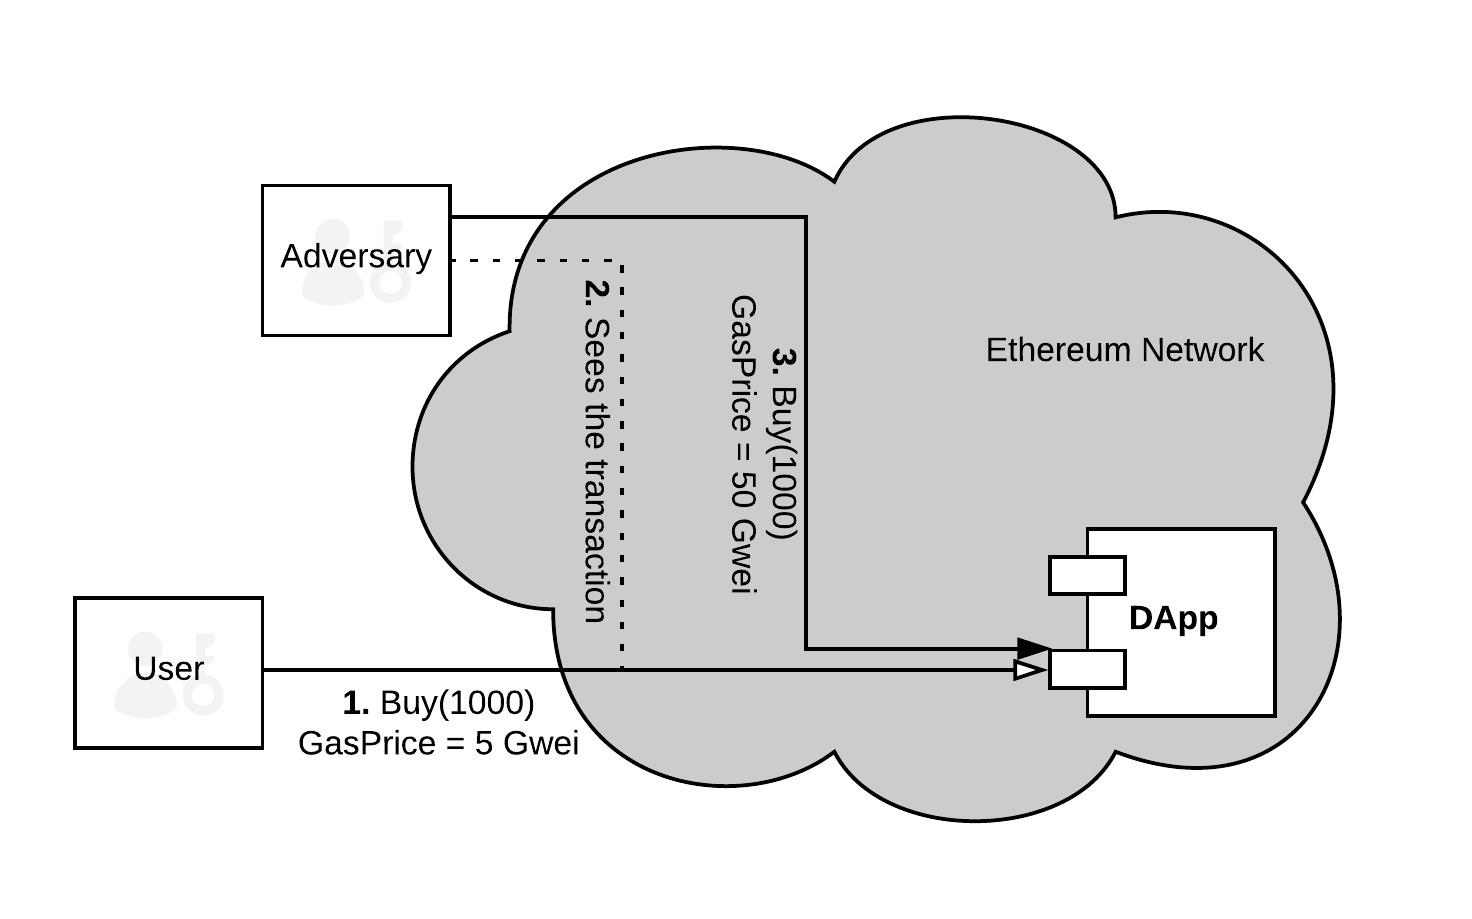
\includegraphics[width=0.7\linewidth]{figures/Regular_frontrunning.png}
\caption{The Adversary up on seeing the Buy order, sends his own buy order with higher gas to front-run the first order. \label{fig:RegularFrontrunning}} 
\end{figure}
%https://www.lucidchart.com/invitations/accept/f8ca2662-5269-425d-9deb-deb14af2aac7


Designing truly decentralized exchanges, where the orderbook is implemented directly on a public blockchain, is being pursued by a number of projects [\textblue{cite github page}]. These designs generally face the following attack (illustrated in Figure~\ref{fig:RegularFrontrunning}). An adversary can monitor the network with a full node for pending \textit{buy} (or \textit{sell}) transactions which could increase (or \textit{decrease}) the future price of the asset. A front-runner can send a competing orders with a higher gas price, and hope to have her transactions mined ahead of the original pending transaction. The benefits of doing this vary. If the original bid is a large market order (\ie it will execute at any price), the adversary can front-run a pair of limit orders that will bid near the best offer price and offer at a higher price. If these execute ahead of the market order, the front-runner profits by scalping the price of the shares. If the adversary has pre-existing offers likely to be reached by the market order, she could front-run a cancelation and a new offer at a higher price. A simpler attack would be to guage the demand for trades at a given price by the number of pending orders, and to front-run at the same price in hopes that the market demand is the result of accurate new market information. Miners are in the best position to conduct these attacks as they hold fine-grained control over the exact set of transactions that will execute and in what order and can mix in their own (late) transactions without broadcasting them. Miners do however have to commit to what their own transactions will be before beginning the proof of work required to solve a block. 

% Front-running can also occur in non-financial smart contracts. As an example, a smart contract which adds all the participants to a party invite list could only be closed by the smart contract owner. In this case, when the owner sends the transaction to close the list, a miner can include his own list of participants before the close transaction in the block he mines. This is an issue with the design of the smart contracts and is known as transaction-ordering dependence vulnerability~\cite{luu2016making}. 

Bancor is another Ethereum-based application that allows users to exchange their tokens without any counter-party risk. This protocol aims to solve the cryptocurrency liquidity issue by introducing \textit{Smart Tokens}~\cite{hertzog2017bancor}. Smart tokens are ERC20-compatible and can be bought or sold through a DApp-based dealer that is always available and implements a market scoring rule to manage its prices. Doing so, Bancor provides continuous liquidity for digital assets without relying on brokers to match buyers with sellers. Implemented on the Ethereum blockchain, when transactions are broadcast to the network, they sit in a pending transaction pool known as \textit{mempool} waiting for the miners to mine them. Since Bancor handles all the trades and exchanges on the Ethereum blockchain (unlike other existing decentralized exchanges), these transactions are all visible to the public for some time before being included within a block. This leaves this blockchain-based decentralized exchange vulnerable to the blockchain race condition attack as attackers are given enough time to front-run other transactions \textblue{and gain favorable profits}~\cite{BancorIs7:online}. Researchers have shown and implemented a proof of concept code to front-run Bancor as a regular non-miner user~\cite{NewTab13:online}.

% = = = 

\subsection{Crypto-Collectibles Games}

The second category of DApp in Table~\ref{tab:top25DApps} is crypto-collectables. Consider Cryptokitties,\footnote{Cryptokitties website \url{https://www.cryptokitties.co/}} the most active DApp in this category and third most active overall. Each cryptokitty (see Appendix~\ref{app:cryptokitty}) is a cartoon kitten with a set of unique features to distinguish it from other cryptokitties, some features more rare and harder to obtain. They can be bought, sold, or bred with other cryptokitties. At the Ethereum level, the kitty is a token implemented with \textit{ERC-721: Non-Fungible Token Standard}~\cite{erc721}. The market cap of cryptokitty tokens peaked at more than 6 million dollars in the first few months their launch, however, has declined since. ERC-721 are similar enough to ERC-20 tokens that they can be listed on exchanges setup for ERC-20. To buy a cryptokittie, the user sends the following bid transaction: \texttt{bid(uint256 \_tokenId)}. It contains the cryptokittty's ID which can be found either on their website or on the ERC721 token smart contract. \textblue{This is similar to open auctions, bid value and the object bidding on is visible to the network and any user could be easily front-run by sending the same transaction with higher gasPrice to replace the initial bidder.}
% https://etherscan.io/tx/0x62a76b7e345e8abd463487d0348c118a9314b197024e090fee7b1fbce434da40

% The blue above needs expansion with further details.

% = = = 

\subsection{Gambling.} 

The third category of DApp in Table~\ref{tab:top25DApps} is gambling services. While a large category of gambling games are based on random outcomes, DApps do not have unique access to an unpredictable data stream to harvest for randomness. Any candidate (such as block headers) source of randomness is accessible to all DApp functions and can also be manipulated to an extent by miners.

\textsf{Fomo3D} is an example of a game style (known as \textsf{Exit Scam}\footnote{\url{https://exitscam.me/play}}) not based on random outcomes, and it is the most active game on Ethereum in our sample. The aim of this game is to be the last person to have purchased a ticket when a timer goes to zero in a scenario where anyone can buy a ticket and each purchase increases the timer by 30 seconds. Many speculated such a game would never end but on August 22, 2018, the first round of the game ended with the winner collecting 10,469 Ether\footnote{The first winner of Fomo3D, won 10,469 Ether \url{ https://etherscan.io/tx/0xe08a519c03cb0aed0e04b33104112d65fa1d3a48cd3aeab65f047b2abce9d508}} equivalent to \$2.1M USD at the time. 
Blockchain forensics indicate a sophisticated winning strategy to frontrun new ticket purchases~\cite{fomo3dhacker} that would reset the counter. The winner appears to have started by deploying some high gas consumption DApps unrelated to the game. When the timer of the game reached about 3 minutes, the winner bought 1 ticket and then sent multiple high gasPrice transactions to her own DApps. These transactions congested the network and bribed miners to prioritize them ahead of any new ticket purchases in \textsf{Fomo3D}. 

%probably needs more work to be good enough. more resources will be out in the coming days!

% Is this the same as order flooding in HFT?

% = = = 

\subsection{Name Services.}\label{sec:ens}

The final category in Table~\ref{tab:top25DApps} is name services, which are primarily aimed at displacing central parties involved in web domain registration (\eg ICAAN and registrars) and resolution (\eg DNS). For simple name services (such as some academic work like Ghazal~\cite{moosavighazal}), domains purchases are transactions and network monitors can front-run other users attempting to register domains. This parallels front-running attacks seen in regular (non-blockchain) domain registration~\cite{sac022en33:online}. \textsf{Ethereum Name Service (ENS)}\footnote{\url{https://ens.domains/}} is the most active naming service on Ethereum. Instead of allowing new  \texttt{.eth} domain names to be purchased directly, they are put up for a sealed bid auction. \textblue{Although sealed auction method is used in ENS implementation, the normal workflow uses \texttt{startAuctionsAndBid()} with the deposit equal or higher than the bid, this information leakage could be used to front-run the transaction with the same bid amount or slightly higher to outbid the initial sealed bid. By doing so the front-runner invalidates the original bid and hence registers the domain name himself.} 
 


%% = = = = = = = = = = = = = = = = = = = = = = = = = = %
% = = = ICOs
% = = = = = = = = = = = = = = = = = = = = = = = = = = = %


\section{Cases of Front-running in ICOs}  \label{sec:ICOsfrontrunning}

There have been more than 3000 ICOs on Ethereum alone, estimated to exceed 75 billion dollars in the first half of 2018~\cite{zetzsche2018ico}. In Table~\ref{top25DApps}, no ICO is represented in the top 25. This is because they tend to be high in activity for a short duration only---namely during their sale. Since no major ICO was active on the day that we sampled \texttt{DAppRadar.com}, the ICO category falls through our sampling method. However we identify this as a major category and study it here. 



%. Needless to say, the importance of ICOs as an application of blockchain requires more in-depth analysis of front-running on these type of DApps. 

%ICOs due to the defined cap is similar to our analogy of a queue line, people would line up to get in and there's an opportunity to front-run. 

%Here we focus on one ICO that our preliminary research showed that there might have been a front-running incident. There is no doubt that similar behaviour could be seen in other instances of ICOs or similar DApps if investigated.

\subsection{\textit{Status.im} ICO}
As discussed in Section~\ref{sec:Front Running on the Blockchains}, capped ICOs are considerable applications to be investigated in terms of the front-running attacks, \textit{Status.im} ICO is such an application. In June 2017, \textit{Status.im}~\cite{statuswhitepaper} started its ICO and reached the predefined cap within 3 hours, resulting in close to 300,000 Ether of funds. In order to prevent few large investments to buy up all the tokens and limit the amount of Ether deposited in an investment, they used a \textit{fair} token distribution method named \textit{Dynamic Ceiling} as an attempt to increase the opprotunity window for smaller investors. They implemented multiple caps --ceiling-- in which, each had a maximum amount that could be deposited in. In this case, every deposit was checked by the smart contract and the exceeding amount was refunded to the sender while the accepted amount was sent to their multi-signature wallet address~\cite{statusicoanalysis}. 

During the time the ICO was open for participation, there were reports of Ethereum network being unusable and transactions were not confirming. Further study showed that some mining pools might have been manipulating the network for their own profit. In addition, there were many transactions sent with a higher gas price to front-run other transactions, however, these transactions were failing due to the restriction in the ICO smart contract to reject any transactions with higher than 50 \textit{GWei} gas price (as an attempt to prevent the known front-running behaviour).

\begin{figure}[h]
\centering
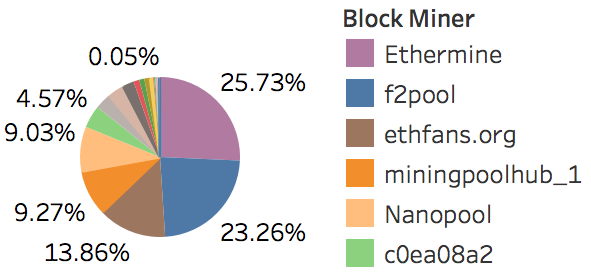
\includegraphics[width=0.5\linewidth]{figures/Mining_pool_ratio.png}
\caption{The percentage of Ethereum blocks mined between block 3903900 and 3908029, this is the time frame in which Status.im ICO was running. This percentage roughly shows the hashing power ratio each miner had at that time. \label{fig:mining_pool_ratio}} % IS THIS STATEMENT CORRECT?
\end{figure}

\subsection{Data Collection and Analysis}
According to the analysis we carried out, it was discovered that the F2Pool, an Ethereum mining pool that had around 23\% of the mining hash rate at the time (Figure ~\ref{fig:mining_pool_ratio}), sent 100 Ether to 30 new Ethereum addresses before Status.im ICO started. On the time the ICO was opened for participation, F2Pool constructed 31 transactions to the ICO token sale smart contract from the addresses they controlled --without broadcasting these transactions to the network-- and used their entire mining power to mine their own transactions and some other potentially failing high gas price transactions.

Ethereum blockchain contains all transaction ever made on Ethereum, however, it is not easy to see the behaviour of the participants and miners solely using the default clients nor online blockchain explorers. In order to get the required data, Ethereum blockchain data should be converted to a queryable format. For this case study, we used open source projects such as Go Ethereum implementation\footnote{Official Go implementation\url{https://github.com/ethereum/go-ethereum}} for the full node, python script for extracting, transforming and loading ethereum blocks, named \texttt{ethereum-etl}~\cite{ethereumetl} and Google BigQuery\footnote{\url{https://cloud.google.com/bigquery/}}. Using this software stack, we were able to query for all the transactions and blocks within the window of Status.im ICO for further analysis which was mainly done by data analysis tool \texttt{Tableau}\footnote{\url{https://www.tableau.com/}}. A copy of this dataset and the initial findings can be found in our Github repository\footnote{\url{github.com / ANONYMOUS}}. 

As shown in Figure~\ref{fig:Transactions_miners_while_status_ico_cut}, most of the top miners in the mentioned time frame, have mined almost the same number of failed and successful transactions which were directed toward Status.im token sale, however F2Pool's transactions indicate their successful transactions were equivalent to 10\% of the failed transactions, hence maximizing the mining rewards on gas, while censoring other transactions to the token sale smart contract. The terminology used here is specific to smart contract transactions on Ethereum, by \textit{``failed transaction''} we mean the transactions in which the smart contract code flow rejected and threw an exception and by \textit{``successful transaction''} we mean the transactions that went through and received tokens from the smart contract. 


\begin{figure}[h]
\centering
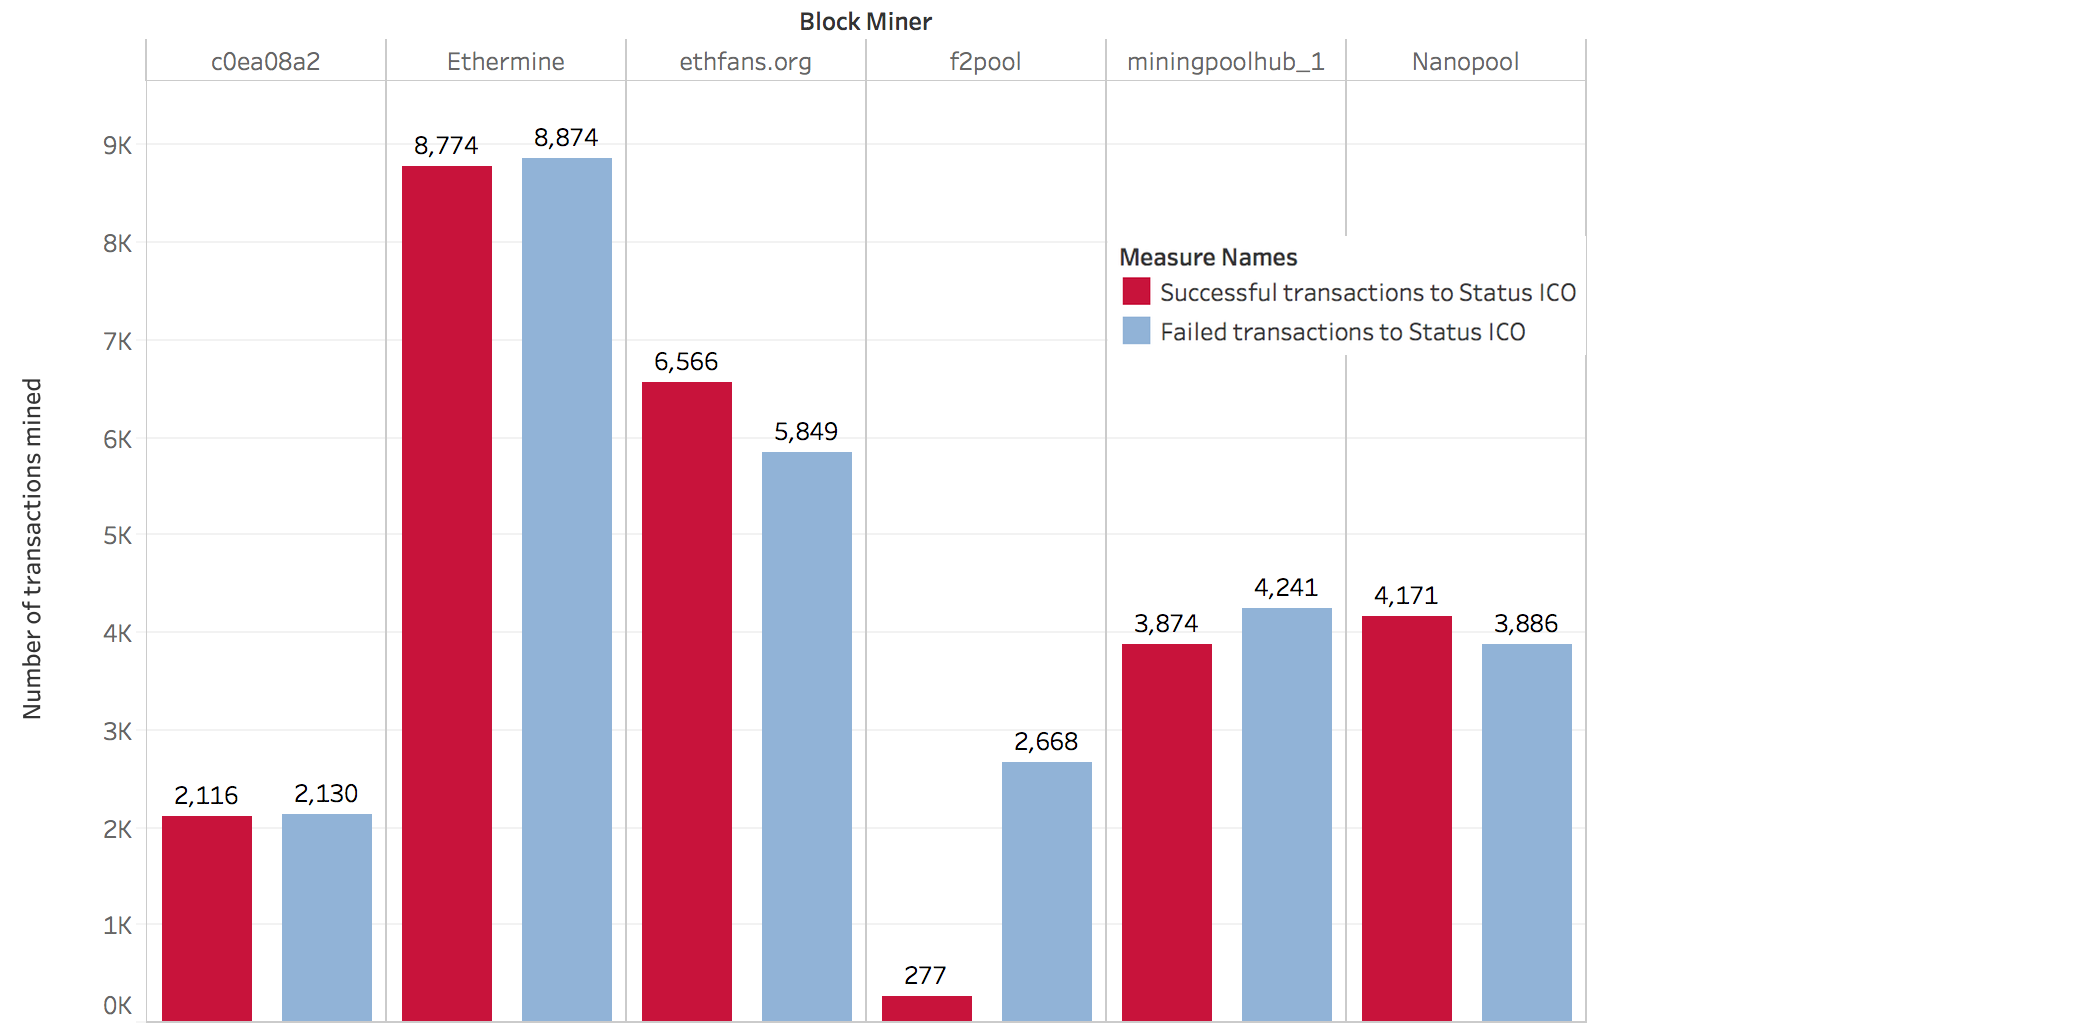
\includegraphics[width=0.7\linewidth]{figures/Transactions_miners_while_status_ico_cut_only_icotx.png}
\caption{This chart shows the miners behaviour on the time window that Status.im ICO was running. It is clear that the number of successful transactions mined by F2Pool do not follow the random homogeneous pattern of the rest of the network. \label{fig:Transactions_miners_while_status_ico_cut}} 
\end{figure}

% make pie charts for each mining pool, all non-status-ico transactions vs success-ico-transactions vs failed-ico=transactions

By tracing the transactions from these 30 addresses, we found explicit Interference of the F2Pool\footnote{F2Pool Ethereum address was identified by their mining reward deposit address \url{https://etherscan.io/address/0x61c808d82a3ac53231750dadc13c777b59310bd9}} in this scenario. As shown in Figure~\ref{fig:f2poolfront-run}, the funds deposited by F2Pool in these addresses were sent to Status.im ICO and mined by F2Pool themselves, where the dynamic ceiling algorithm refunded a portion of the deposited funds back to these addresses, these funds were sent back to F2Pool main address a few days after. 

\begin{figure}[h]
\centering
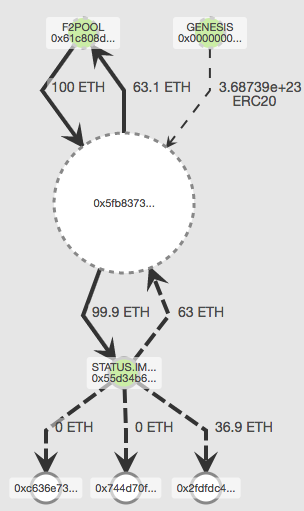
\includegraphics[width=0.7\linewidth]{figures/F2Pool_transactions_to_StatusICO_and_Refunds.png}
\caption{F2Pool prior to Status.im ICO deposited 100 Ether in multiple new Ethereum addresses. On the time of the ICO they sent these deposits to Status ICO smart contract and prioritized mining of these transactions in their mining pool, this was to overcome the dynamic ceiling algorithm of the token sale smart contract. Later on they sent the refunded Ether back to their own address. [Graph made using Blockseer.com] \label{fig:f2poolfront-run}}
\end{figure}


Although this incident does not involve transaction reordering in the blocks, it shows how miners can modify their mining software to behave in a certain way to front-run other transactions and gain monetary profit. The dataset used for this analysis can be found on our GitHub repository.\footnote{Front-running Status.im ICO dataset: \url{http://github.com/ANONYMOUS}}. 
%______________________________________________________________%


% = = = = = = = = = = = = = = = = = = = = = = = = = = %
% = = = Mitigations
% = = = = = = = = = = = = = = = = = = = = = = = = = = %

\section{How to stop Front-running?} %We have the applicability of the solutions inline.

In the traditional markets, front-running is considered unethical and illegal. In the blockchain space, the designers of the decentral applications cannot rely on the justice system for preventing unethical behavior, and they must assume that each participant in the network acts rationally in their own self-interest, the application will be operating in an adversarial environment~\cite{0xfrontrunning:online}.
A few decentral exchange projects such as \textit{EtherDelta} and \textit{0xProject}~\cite{warren20170x}, have proposed solutions for front-running, which is off-chain order books. The methods discussed within these projects prevent blockchain network participants from front-running the orders as the orders are private and not known to the network and will not be broadcasted. However they are introducing third parties, \eg relayers in 0xproject, to be managing the orders with the promise not to reorder or front-run other orders. 

\emph{Traditional Front-running Prevention Methods}. There are debates in traditional markets regarding the fact that front-running is considered to be a form of insider trading which deemed to be illegal. Traditional methods to prevent front-running mainly involves after the fact investigation and legal action against the front-runners~\cite{LexisNexisLawSuit}. As mentioned in section~\ref{traditionalFrontrunning}, defining front-running and educating the employees were the first step taken to prevent such issues in traditional markets, however, front-running became less likely to happen mainly because of the high fine and lawsuits against firms who behaved in an unethical way. Other methods such as dark pools~\cite{zhu2014dark, buti2011diving} and sealed bids~\cite{radner1989sealed} were discussed and implemented in a variety of regulated trading systems. 

The traditional methods to prevent front-running does not apply to blockchain applications, as mainly they are based on central enforcement and limitations, also in case of blockchains the actors who are front-running could be anonymous and the fear of lawsuits would not apply. \\

There are two main approaches to prevent front-running blockchains: one to design a blockchain that is front-run resistant, and the other to design the application logics in a way that front-running is not possible. 
%______________________________________________________________%
\subsection{Front-run Resistant Blockchain}
There are technical difficulties to achieve such solutions as there are unknown factors within such network designs and requires testing every corner and edge case scenarios. In this section, we describe the potential solutions using which, one can design and implement a decentral application that is resistant to front-running.

\subsubsection{Design Decision \#1: Fixed Transaction Ordering\newline}
One possible solution to fix current blockchains in regards to transaction reordering by miners has been proposed by da Silva~\etal~\cite{fixedordering2018silva}. This solution consists of an algorithm, known as Fixed Transaction Ordering and Admission (FTOA) algorithm, in the consensus protocol that enforces the order of the transactions in the mined blocks.

\subsubsection{Design Decision \#2:Privacy-Preserving Blockchain\newline}
Market participants are concerned about revealing information on their past trades, purchases, income, or liquidity needs. Privacy is a basic human right, that being said, there are limitations to the functionality of a system designed to preserve full privacy. However other than past transactions, real-time transactions would leak information about the sender or the intention of the order that could lead to front-running attacks. Privacy-preserving blockchains try to solve the initial issue by keeping all the details of the transactions private (in some extent~\cite{miller2017empirical, kappos2018empirical}). 
As an example, ZCash~\cite{hopwood2016zcash}, uses two distinct type of addresses, transparent addresses and shielded addresses. Transparent addresses work similar to Bitcoin transactions, fully transparent about the sender and receiver addresses, the amount and included data. However shielded addresses are private and do not leak any information, this is great for privacy but not good for smart contracts capabilities. Smart contract functionality requires verification by the miners which require to know the input, functionality, and output of smart contracts to be able to determine if the transaction is valid. Albeit by using cryptographic primitives such as zero-knowledge proofs this issue could also be resolved~\cite{kosba2016hawk}. 

\subsubsection{Design Decision \#3: Dual Authoring\newline} Loopring is an open protocol proposed by Wang~\etal to build decentralized exchanges~\cite{wang2018loopring}. This protocol operates a hybrid model with off-chain order management and communication while only the order matching takes place on the chain. In this protocol, the orders are grouped in \emph{ring orders} immediately after they are sent by the users. Next, the required signatures are provided by a miner and owner of the order, see Figure~\ref{fig:vulnerable_loopring}. Eventually, the ring miner sends the \emph{submitRing transaction} to the Loopring Smart Contract (LPSC) for verification and settlement. While the \emph{submitRing transaction} sits unconfirmed in the mempool, any front-runner can create a copy of this transaction with his address instead of the ring miner's address and then sign the hash of the ring using his own private key. By paying a higher gasPrice, block miners choose the front-runner's transaction instead of the original \emph{submitRing transaction}. 
To solve this issue, the new version of Loopring protocol uses the \emph{dual-authoring} scheme. This solution sets two levels of authorization for orders - one for settlement, and one for order matching. As it can be seen in Figure~\ref{fig:not_vulnerable_loopring}, each owner of an order generates a pair of public key (auth-address) and private key (auth-key), which are different from his address and its corresponding private key. These auth-keys are used to sign the hash of the ring and will further prevent anyone from regenerating the same \emph{submitRing transaction}. The reason is that the auth-keys are only known to the miner of the ring as they are not part of the on-chain transaction. Doing so, it is assured that (i) the orders are not modified (because they are signed by the owner), (ii) no other miner can mine the ring (because the miner's address is signed by the initial miner), and no user can front-run the \emph{submitRing transaction} (because other users do not have access to the auth-keys and hence are not able to generate new transactions with auth-keys signatures on them).



\begin{figure}[h]
\centering
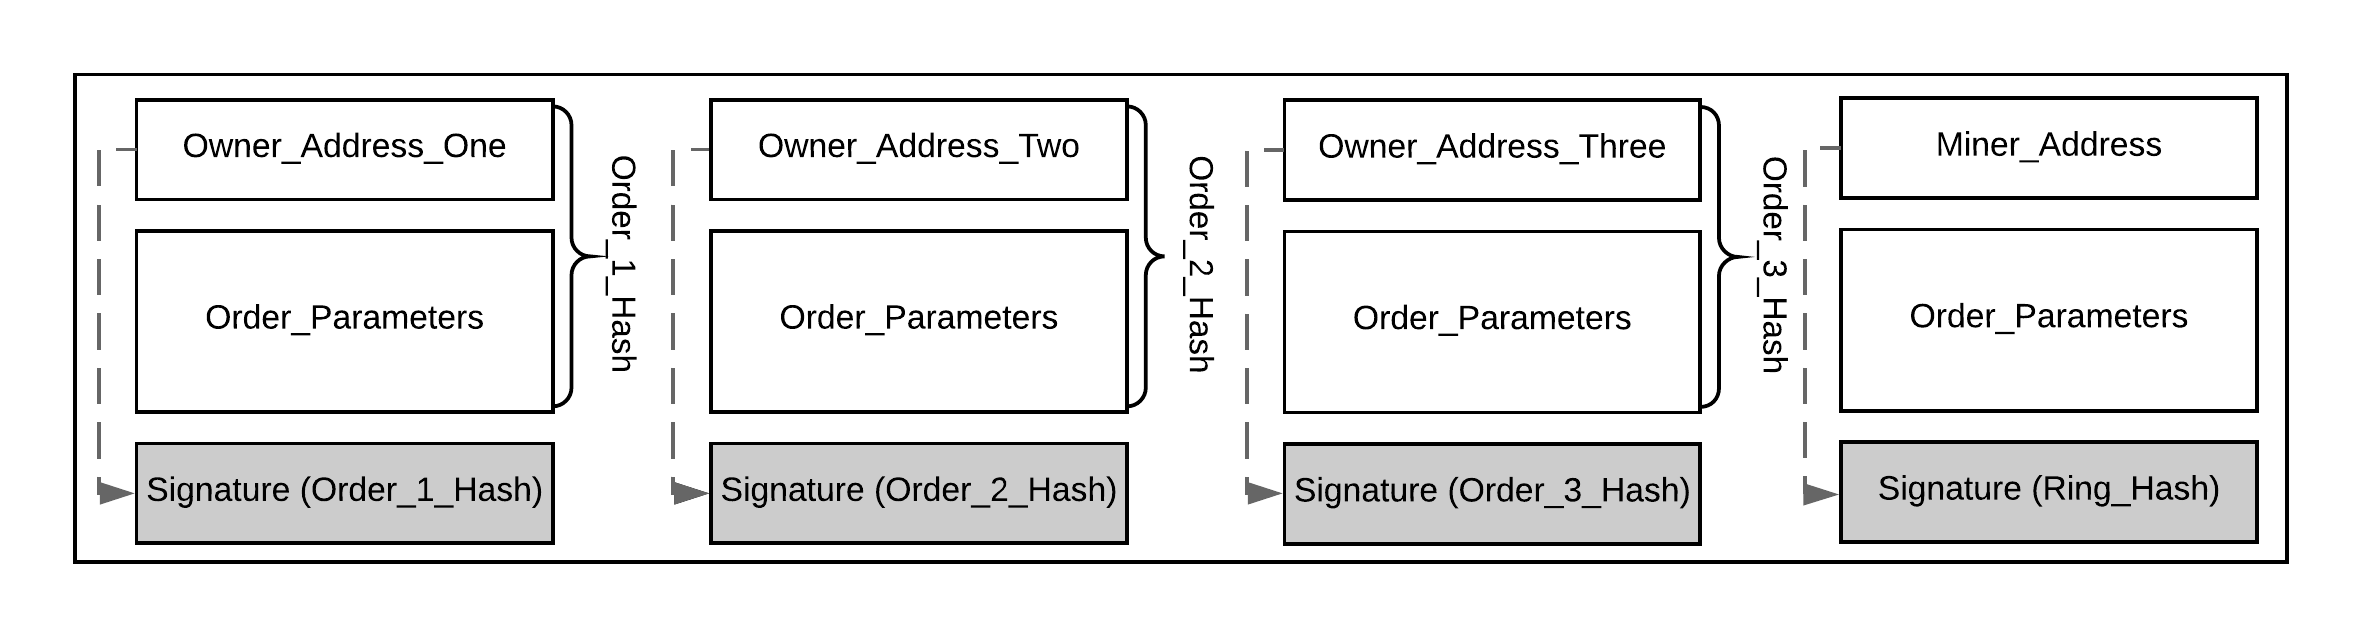
\includegraphics[width=0.7\linewidth]{figures/Vulnerable_Loopring.png}
\caption{\emph{submitRing} Transaction in the old version of the Loopring protocol. Any user can regenerate this transaction by replacing the miner's address with his address and signing the hash of the ring using his private key. \label{fig:vulnerable_loopring}}
\end{figure}
%https://www.lucidchart.com/invitations/accept/33d38ce9-4660-4743-806d-45c72f7e8393
\begin{figure}[h]
\centering
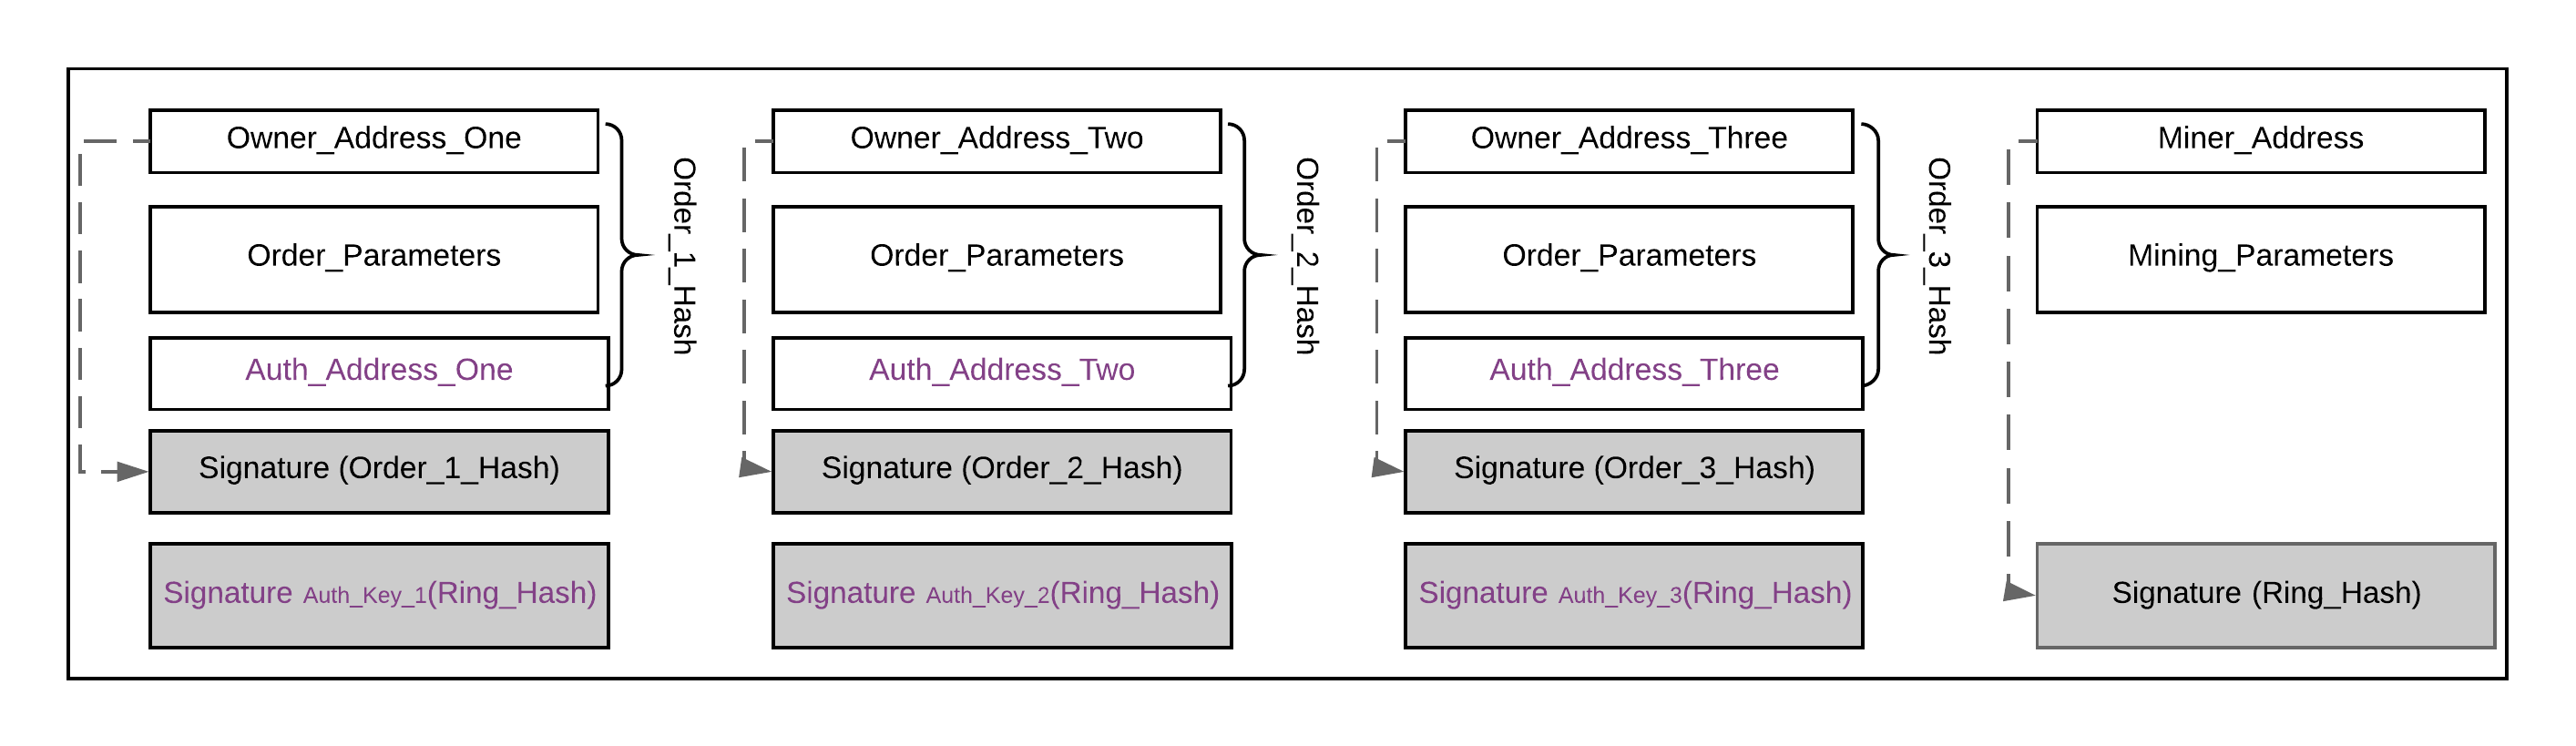
\includegraphics[width=0.7\linewidth]{figures/Dual_Authoring_Loopring.png}
\caption{\emph{submitRing} Transaction in the new version of the Loopring protocol. Other users cannnot regenerate this transaction as they do not access auth-keys and hence are not able to create the signatures. \label{fig:not_vulnerable_loopring}}
\end{figure}
%https://www.lucidchart.com/invitations/accept/8dee869c-482c-433f-a901-8d041a1dc526
%______________________________________________________________%
\subsection{Application Design to Prevent Front-running}

Another method to prevent front-running activities is to design the applications in such a way that there is no information leakage to the malicious parties to enable them to front-run other users.
Followings discuss a few techniques which can be used by the DApp developers while designing the systems to mitigate front-running issues.

\subsubsection{Design Decision \#1: Commitment Scheme\newline} \label{CommitmentScheme}
The commitment scheme is a cryptographic primitive that enables one to commit to a value --binding-- (\eg statement, document, data, \etc) while keeping it a secret and reveal the committed value on a later time~\cite{brassard1988minimum}. The commitment scheme is a robust method to prevent information leakage from the sensitive transactions. This could be done by simply submitting the hash value of the committed data to a smart contract and later on revealing the values linked to the committed hash, see Figure~\ref{fig:commitReveal}. 
In the case of decentral exchanges, the user can send a commit transaction which will be cryptic to network participants but will act as a placeholder in the queue for the user, after the transaction is mined, the user sends reveal transaction revealing the order details which will be executed in a fair order. This method is not perfect, depending on the DApp design, either the order is collateralized, that means the commitment transaction includes the funds required for fulfilling the order, which will leak some information about the order, or is not collateralized and opens up the possibility of user never revealing the commitment, which will be vulnerable to Denial-of-Service attacks. 
Another use of such a commitment scheme is in decentralized naming systems, such as Namecoin, Ethereum Name Service (ENS). In this case, a user sends a commit transaction, which commits to the name hash, similar to a sealed bid. Once the transaction is confirmed and the grace period is over, the user sends a reveal transaction revealing the bid and also the details of the requested domain~\cite{kalodner2015empirical}. Using this scheme, one is able to hide information from the adversarial parties in the system and prevent them from front-running. A similar approach applies to on-chain voting as well ~\cite{adChainPLCRVoting}, using sealed votes, voters can make sure their votes are hidden until a later date, however, their participation and weight of the vote are publicly known. 
Other than the collateralization issue for the commit and reveal scheme, another obvious issue is the participatory factor. For anyone watching the DApp address, there will be a direct transaction from the user to the DApp address, It will be obvious that a specific address has participated in the auction or the DApp using a commit and reveal scheme, but the details are hidden through the scheme. Both these issues, albeit hiding the details of the order and preventing direct front-running, leak information to other participants which could lead to more sophisticated front-running attacks depending on the application design. On the other note, these method has some drawbacks, the user experience is not smooth and one might forget to reveal the committed transaction. In the ENS commit-reveal process, if one forgets to reveal in the reveal phase, the committed funds are burnt and inaccessible thereafter. Also, this scheme means two transactions are required for a functionality which makes it more expensive to run.

\begin{figure}[h]
\centering
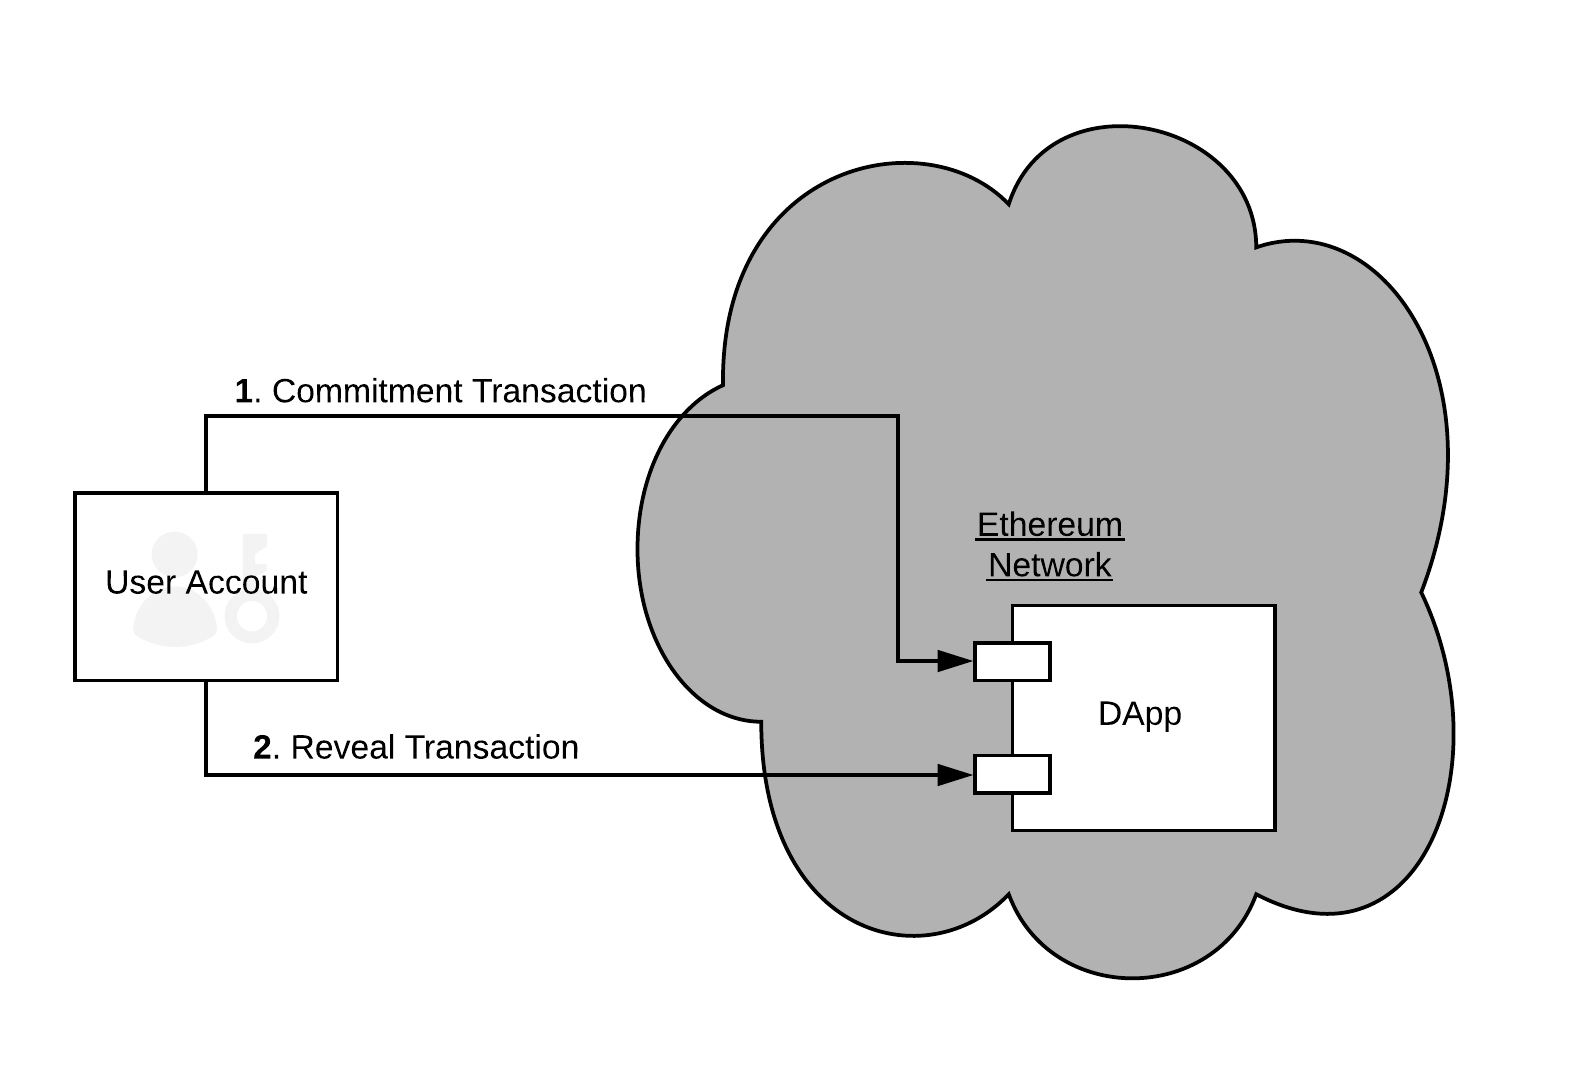
\includegraphics[width=0.5\linewidth]{figures/commit-reveal.png}
\caption{Commit and Reveal. User sends a commitment transaction with the hash of the data, After the commitment period is over, user sends her reveal transaction to the DApp revealing the information that matches the commitment. \label{fig:commitReveal}}
\end{figure}
%https://www.lucidchart.com/invitations/accept/3cd4c865-83d4-4c71-9a4a-f2e870f2db2c

\subsubsection{Design Decision \#2: Submarine Commitments\newline}\label{submarineCommits}
Submarine Commitments~\cite{breidenbach2018enter, submarinesendHD} are similar to the commitment schemes with some key differences such as hiding participatory factor and being fully collateralized. With submarine send, it is possible to hide sender, receiver, value, and data, the commitment transaction is identical to a transaction to a newly generated address. Submarine sends could be a solution for sealed-bid auctions on the blockchain to hide the existence of the bids for other participants. 

The details of how Submarine commitments work is outside the scope of this paper, however in short, using the way Ethereum transactions are constructed and ECDSA ECRecover functionality it is possible to generate one outgoing transaction from an address of which no private key exists. By constructing a transaction from that address to the DApp and funding that address we fulfill the commitment phase and by revealing the details and broadcasting the constructed transaction we reveal the commitment ~\cite{libsubmarine}, see Figure~\ref{fig:LibSubmarine}. However, this could be designed in other ways to suit the need of the DApp. Drawbacks of this scheme are similar to ~\ref{CommitmentScheme}, with an addition of two more transactions to finalize the functionality, which results in more cost and complicated user experience.

\textblue{Cite Princeton paper on Namecoin for frontrunning mitigation using commit/reveal.}


\begin{figure}[h]
\centering
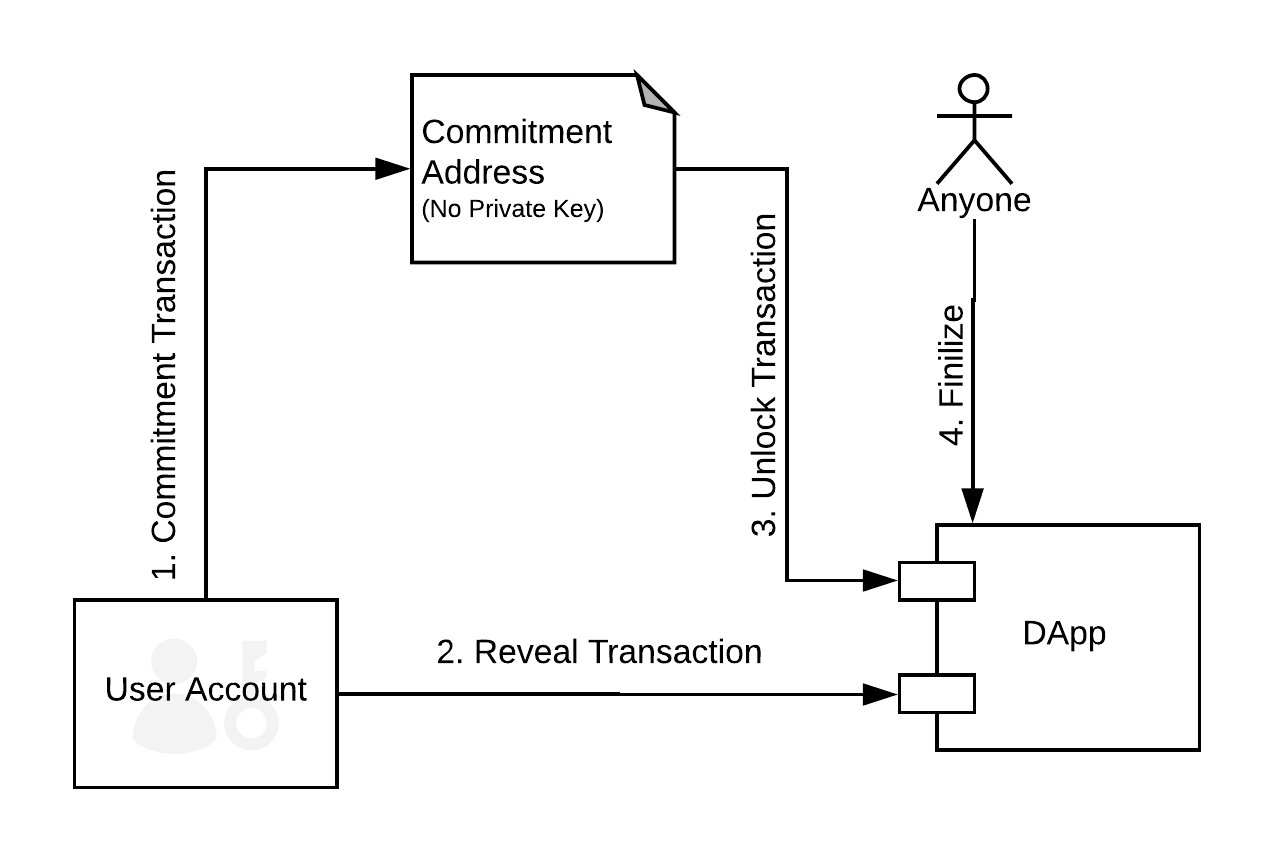
\includegraphics[width=0.5\linewidth]{figures/LibSubmarine.png}
\caption{Submarine Send~\cite{libsubmarine}. User generates an \textit{Unlock} transaction from which the commitment address is retrieved. By funding the \textit{commitment address}, user is committed to the unlock transaction. After the commitment transaction, in the reveal phase, user sends the \textit{reveal transaction} to the DApp and then after she can broadcast the Unlock transaction to unlock the funds in the commitment address. Finally after the "Auction'' is over, anyone can call \textit{Finalize} function to finalize the process.  \label{fig:LibSubmarine}}
\end{figure}
%https://www.lucidchart.com/invitations/accept/3a259b74-1162-4fb5-8023-eb0311018295


\subsubsection{Design Decision \#3: Logic Specific Solutions\newline}
There is no perfect generic solution to this issue as of now, however, to prevent front-running, one can design the application in a way that it is not possible to be front-run:

\noindent\emph{Eliminating Time-Order Dependency:} The applications can be designed not to rely on the time for the orders to be executed. For example when designing a decentral exchange, one can use \emph{the call market} design instead of a time-sensitive order book. In a call market design, the arrival time of the orders does not matter as they are executed in batches~\cite{clark2014decentralizing}. 

\noindent\emph{Disincentivizing Front-running Actors:} This solution, which is economic rather than technical, is to disincentives the miners by paying them the fees. If the application is designed in a way that the fees of the orders are sent to the miner of the block, he would have less incentive to front-run the orders as he already gains enough financial benefit from acting fairly and executing the transactions on their correct order. For example, Malinova~\cite{malinova2017market} proposes a design for a decentral exchange which uses economic models in their trading market design to make front-running expensive and more costly than profitable. 


% one solution could be to remove multiple actors, meaning that on each "play" (order), the smart contract would be the market maker. it does not matter if there are multiple similar orders. similar to PoC of Velocity~\cite{eskandari2017feasibility}. Although there are other concerns about this specific design but not for front-running.

Going back to Table~\ref{tab:top25DApps}, some DApps facilitate different methods to mitigate front-running issues. As an example, LocalEthereum, an escrow-based exchange, uses challenge random values from the website to be included in the signature of the transaction (See ~\ref{code:localethereum}), hence removing any possibility of replay attack or the possibility of any other address sending the similar order.

%Possibly remove this code snippet due to page limit . don't forget to remove the refrence to it ^
\begin{lstlisting}[basicstyle=\scriptsize\ttfamily,caption={Code snippet from LocalEthereum smart contract. Values V,R and S are set by LocalEtherem to have a valid signature, also the tradeHash uses buyer and seller addresses, mitigating the possibility of front-running by a third party.},label={code:localethereum},float]
    function createEscrow(bytes16 _tradeID, address _seller, address _buyer, uint256 _value, uint16 _fee,
					uint32 _paymentWindowInSeconds, uint32 _expiry, uint8 _v, bytes32 _r, bytes32 _s) 
        payable external {
        bytes32 _tradeHash = keccak256(abi.encodePacked(_tradeID, _seller, _buyer, _value, _fee));
	...
        // A signature (v, r and s) must come from localethereum to open an escrow
        bytes32 _invitationHash = keccak256(abi.encodePacked(
            _tradeHash,
            _paymentWindowInSeconds,
            _expiry
        )); 
\end{lstlisting}

%Proof of burn methods ? 


%TODO: inline talk about what these solutions are good for and if they fit Status ICO


%______________________________________________________________%
\section{Concluding Remarks}



% Could talk about future work on a tool / a framework to detect front-running


%\subsubsection*{Acknowledgements.}
